\documentclass[12pt]{article}

\usepackage{amsmath,amsthm,amsfonts,amssymb,amsxtra}
\usepackage{pgf,tikz}
\usepackage{multicol}
\usetikzlibrary{arrows}
\renewcommand{\theenumi}{(\alph{enumi})} 
\renewcommand{\labelenumi}{\theenumi}

\pagestyle{empty}
\setlength{\textwidth}{7in}
\setlength{\oddsidemargin}{-0.5in}
\setlength{\topmargin}{-1.0in}
\setlength{\textheight}{9.5in}

\theoremstyle{definition}
\newtheorem{problem}{Problem}

\makeatletter
\newcommand*{\radiobutton}{%
  \@ifstar{\@radiobutton0}{\@radiobutton1}%
}
\newcommand*{\@radiobutton}[1]{%
  \begin{tikzpicture}
    \pgfmathsetlengthmacro\radius{height("X")/2}
    \draw[radius=\radius] circle;
    \ifcase#1 \fill[radius=.6*\radius] circle;\fi
  \end{tikzpicture}%
}
\makeatother

\begin{document}

\noindent{\large\bf MATH 122}\hfill{\large\bf Final Exam}\hfill{\large\bf
  Fall 2016}\hfill{\large\bf Page 1/8}\hrule

\bigskip
\begin{center}
  \begin{tabular}{|ll|}
    \hline & \cr
    {\bf Name: } & \makebox[12cm]{\hrulefill}\cr & \cr
    {\bf VIP ID:} & \makebox[12cm]{\hrulefill}\cr & \cr
    \hline
  \end{tabular}
\end{center}
\begin{itemize}
\item Write your name and VIP ID in the space provided above.
\item The test has eight (8) pages, including this one, not counting the formula sheet attached at the end.  
\item You may remove the formula sheet as soon as the proctor instructs so.
\item Credit for each problem is given in parentheses at the right of the problem number. 
\item You must show sufficient work to justify all answers except on multiple-choice questions.  Correct answers with inconsistent or no work will not be given credit.
\item No books or notes may be used on this test.
\item No scratch paper is allowed.  You may use the last page of this booklet for that purpose.
\item An approved calculator may be used on this test.
\end{itemize}
\hrule

\begin{center}
  \begin{tabular}{|c|c|c|}
    \hline
    &&\cr
    {\large\bf Page} & {\large\bf Max.~points} & {\large\bf Your points} \cr
    &&\cr
    \hline
    &&\cr
    {\Large 2} & \Large 16 & \cr
    &&\cr
    \hline
    &&\cr
    {\Large 3} & \Large 12 & \cr
    &&\cr
    \hline
    &&\cr
    {\Large 4} & \Large 28 & \cr
    &&\cr
    \hline
    &&\cr
    {\Large 5} & \Large 20 & \cr
    &&\cr
    \hline
    &&\cr
    {\Large 6} & \Large 12 & \cr
    &&\cr
    \hline
    &&\cr
    {\Large 7} & \Large 12 & \cr
    &&\cr
    \hline\hline
    &&\cr
    {\large\bf Total} & \Large 100 & \cr
    &&\cr
    \hline
  \end{tabular}
\end{center}

\newpage

%%%%%%%%%%%%%%%%%%%%%%%%%%%%%%%%%%%%% Page 2
\noindent{\large\bf MATH 122}\hfill{\large\bf Final Exam}\hfill{\large\bf
  Fall 2016}\hfill{\large\bf Page 2/8}\hrule

\bigskip

\begin{problem}[4 pts]
The graph below is a representation of which of the following functions?
\begin{multicols}{2}
\begin{center}
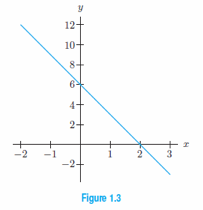
\includegraphics{1graph2.png}
\end{center}
\begin{itemize}
\item[\radiobutton] $y=6x+6$
\item[\radiobutton] $y=-3x+6$
\item[\radiobutton] $y=-3x+2$
\item[\radiobutton] $y=6x-2$
\end{itemize}
\end{multicols}
\end{problem}

\hrule
\begin{problem}[4 pts]
You are to receive three equal payments of \$2000 each, paid once per year starting now. You can assume a 5\% interest rate, compounded continuously. The future value of the payments, on the day you receive the final payment, is:
\begin{itemize}
\item[\radiobutton] $6000 e^{0.05 \cdot 3}$
\item[\radiobutton] $6000 e^{0.05 \cdot 2}$
\item[\radiobutton] $2000 e^{0.05 \cdot 3} + 2000 e^{0.05 \cdot 2} + 2000 e^{0.05 \cdot 1}$
\item[\radiobutton] $2000 e^{0.05 \cdot 2} + 2000 e^{0.05 \cdot 1} + 2000$
\end{itemize}
\end{problem}
\hrule

\begin{problem}[4 pts each]
Evaluate the following integrals.
\begin{enumerate}
\item $\displaystyle{\int_{0}^{4} \ln(y^2 + 1) \, dy} = $
\item $\displaystyle{\int_{10}^{103} 9xe^{30x^2}\, dx = }$
\vspace{7cm}
\end{enumerate}
\end{problem}

\newpage

%%%%%%%%%%%%%%%%%%%%%%%%%%%%%%%%%%%%% Page 3
\noindent{\large\bf MATH 122}\hfill{\large\bf Final Exam}\hfill{\large\bf
  Fall 2016}\hfill{\large\bf Page 3/8}\hrule

\bigskip

\begin{problem}[4 pts]
If the graph below is that of $f'(x)$, which of the following statements is true concerning the function $f(x)$?
\begin{multicols}{2}
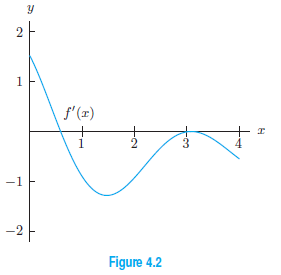
\includegraphics{3graph2}
\vspace{2cm}

\begin{itemize}
\item[\radiobutton] The derivative is zero at two values of $x$, both being local maxima.
\item[\radiobutton] The derivative is zero at two values of $x$, one is a local maximum, while the other is a local minimum.
\item[\radiobutton] The derivative is zero at two values of $x$, one is a local maximum on the interval, while the other is neither a local maximum nor a minimum.
\item[\radiobutton] The derivative is zero at two values of $x$, one is a local minimum on the interval, while the other is neither a local maximum nor a minimum.
\item[\radiobutton] The derivative is zero only at one value of $x$, where it is a local minimum.
\end{itemize}
\end{multicols}
\end{problem}

\hrule
\begin{problem}[4 pts]
Find all local max, min, and inflection points of $f(x) = 2x^3 + 3x^2-180x+9$.
\end{problem}
\vspace{6cm}
\hrule
\begin{problem}[4 pts]
Find the global maximum and the global minimum of $f(x) = 2x^3 - 9x^2$ over the interval $-1 \leq x \leq 6$.
\end{problem}

\newpage

%%%%%%%%%%%%%%%%%%%%%%%%%%%%%%%%%%%%% Page 4
\noindent{\large\bf MATH 122}\hfill{\large\bf Final Exam}\hfill{\large\bf
  Fall 2016}\hfill{\large\bf Page 4/8}\hrule

\bigskip

\bigskip
\begin{problem}[4 pts each]
Find the derivative of the following functions:
\begin{enumerate}
\item $f(x) = \sqrt{\dfrac{1}{x^{39}}}$
\begin{flushright}
  \begin{tikzpicture}
    \draw (-4cm,0.5cm) node {$f'(x)=$};
    \draw (-3cm,-0.2cm) rectangle (5cm,1.2cm);
  \end{tikzpicture}
\end{flushright}
\item $y = 6t^5 - 10\sqrt{t} + \frac{9}{t}$
\begin{flushright}
  \begin{tikzpicture}
    \draw (-4cm,0.5cm) node {$y'(t)=$};
    \draw (-3cm,-0.2cm) rectangle (5cm,1.2cm);
  \end{tikzpicture}
\end{flushright}
\item $f(x) = (2^x + x^5)(3 - \ln x)$
\begin{flushright}
  \begin{tikzpicture}
    \draw (-4cm,0.5cm) node {$f'(x)=$};
    \draw (-3cm,-0.2cm) rectangle (5cm,1.2cm);
  \end{tikzpicture}
\end{flushright}
\item $f(x) = \dfrac{x^8+2}{x}$
\begin{flushright}
  \begin{tikzpicture}
    \draw (-4cm,0.5cm) node {$f'(x)=$};
    \draw (-3cm,-0.2cm) rectangle (5cm,1.2cm);
  \end{tikzpicture}
\end{flushright}
\item $f(x) = \ln \big(8 - e^{-x}\big)$
\begin{flushright}
  \begin{tikzpicture}
    \draw (-4cm,0.5cm) node {$f'(x)=$};
    \draw (-3cm,-0.2cm) rectangle (5cm,1.2cm);
  \end{tikzpicture}
\end{flushright}
\item $f(x) = \big( 6 + \ln x \big)^{0.6}$
\begin{flushright}
  \begin{tikzpicture}
    \draw (-4cm,0.5cm) node {$f'(x)=$};
    \draw (-3cm,-0.2cm) rectangle (5cm,1.2cm);
  \end{tikzpicture}
\end{flushright}
\item $f(x) = 2e^{7x} + e^{-x^6}$
\begin{flushright}
  \begin{tikzpicture}
    \draw (-4cm,0.5cm) node {$f'(x)=$};
    \draw (-3cm,-0.2cm) rectangle (5cm,1.2cm);
  \end{tikzpicture}
\end{flushright}
\end{enumerate}
\end{problem}

\newpage

%%%%%%%%%%%%%%%%%%%%%%%%%%%%%%%%%%%%% Page 5
\noindent{\large\bf MATH 122}\hfill{\large\bf Final Exam}\hfill{\large\bf
  Fall 2016}\hfill{\large\bf Page 5/8}\hrule

\bigskip 

\begin{problem}[4 pts each]
Compute the antiderivative of the following functions:
\item $\displaystyle{\int x^5 (5 - 3x^6)^{12}\, dx =}$
\vspace{2cm}
\item $\displaystyle{\int  6xe^{x^2} \, dx =}$
\vspace{2cm}
\item $\displaystyle{\int \frac{3x^2}{(8x^3-5)^3} dx =}$
\vspace{4cm}
\item $\displaystyle{\int 3x^2 4^{5x^3}\, dx =}$
\vspace{4cm}
\item $\displaystyle{\int \frac{(\ln x)^4}{x} dx =}$
\vspace{4cm}
\end{problem}

\newpage

%%%%%%%%%%%%%%%%%%%%%%%%%%%%%%%%%%%%% Page 6
\noindent{\large\bf MATH 122}\hfill{\large\bf Final Exam}\hfill{\large\bf
  Fall 2016}\hfill{\large\bf Page 6/8}\hrule

\bigskip 

\begin{problem}[4 pts]
The number of acres in a region cleared for farming follows the formula $A = f (t) = 2t^2$, where t is the number of months since the region started to be farmed, and $t$ ranges from $t = 0$ to $t = 10$. Find the \textbf{average rate of change} in the number of acres cleared for farming between $t = 1$ and $t = 4$. 
\begin{itemize}
\item[\radiobutton] 10 acres/month
\item[\radiobutton] 30 acres
\item[\radiobutton] 10 months/acre
\item[\radiobutton] 30 months
\item[\radiobutton] 0.10 months/acre
\end{itemize}
\end{problem}

\hrule

\begin{problem}[4 pts]
What is the \textbf{average value} of $f(x) = \displaystyle{\sqrt{\vphantom{\lvert} 9-x^2}}$ over the interval $0 \leq x \leq 3$? 
\end{problem}
\vspace{4cm}
\hrule

\begin{problem}[4 pts]
For a product, the demand curve is $p=53-q^2$ and the supply curve is $p=3+q^2$, where $q$ is quantity and $p$ is price in dollars per unit. Find the \textbf{producer surplus} when the market is in equilibrium (round your anwer to the nearest dollar).
\end{problem}

\newpage

%%%%%%%%%%%%%%%%%%%%%%%%%%%%%%%%%%%%% Page 7
\noindent{\large\bf MATH 122}\hfill{\large\bf Final Exam}\hfill{\large\bf
  Fall 2016}\hfill{\large\bf Page 7/8}\hrule

\bigskip

\begin{problem}[4 pts]
Find the value of constants $a$ and $b$ so that the minimum of the parabola $f(x) = ax^2 -bx +3$ is at $(1,-1)$.

\vspace{5cm}
\end{problem}
\hrule

\begin{problem}[4 pts]
At a price of \$80 for a half-day trip, a white-water rafting company attracts 300 customers.  Every \$5 decrease in price attracts an additional 30 customers.  What price should the company charge per trip to maximize revenue?
\vspace{7cm}
\hrule

\begin{problem}[4 pts]
The marginal cost of drilling an oil well depends on the depth at which you are drilling; drilling becomes more expensive, per meter, as you dig deeper into the earth.  The fixed costs are one million dollars and, if $x$ is the depth in meters, the marginal costs are $MC(x) = 500 + 12x$ dollars per meter.  Find the \textbf{total cost} of drilling a 400-meter well.
\end{problem}

\end{problem}

\newpage

%%%%%%%%%%%%%%%%%%%%%%%%%%%%%%%%%%%%% Page 8
\noindent{\large\bf MATH 122}\hfill{\large\bf Final Exam}\hfill{\large\bf
  Fall 2016}\hfill{\large\bf Page 8/8}\hrule

\end{document}
